\documentclass[10pt]{IEEE}

\setstretch{1.0}

\begin{document}
\TitleEight
\clearpage

{\small \tableofcontents}
\newpage

\codecolor

\begin{abstract} This document provides a concise user guide and quick-start reference for the Delay-Tolerant Networking (DTN) Satellite Simulator. The simulator integrates orbital mechanics, RF link modeling, and DTN routing protocols into a full-stack research and visualization platform. This guide summarizes installation, basic navigation, simulation configuration, experiment workflows, and troubleshooting procedures. Furthermore, this document also provides a comprehensive overview of the project and its merits.
\end{abstract}
\section{Executive Summary}

This report presents a comprehensive delay-tolerant network (DTN) simulator designed for satellite communications research. The simulator provides a realistic environment for studying DTN routing protocols in satellite constellations with accurate orbital mechanics, RF link modeling, and real-time 3D visualization.

\subsection{Project Overview}

The DTN Simulator is a full-stack application combining:
\begin{itemize}
    \item \textbf{Backend}: Python-based simulation engine with FastAPI REST interface
    \item \textbf{Frontend}: React-based 3D visualization with Three.js
    \item \textbf{Protocols}: Implementation of Epidemic, PRoPHET, and Spray-and-Wait routing
    \item \textbf{Physics}: Realistic orbital mechanics using SGP4/SDP4 propagation
    \item \textbf{RF Modeling}: Complete link budget calculations with weather effects
\end{itemize}

\subsection{Key Features}

\begin{itemize}
    \item Real-time satellite constellation simulation with up to 3600x time acceleration
    \item Three advanced DTN routing protocols with comparative analysis
    \item Realistic RF link budget modeling including weather effects
    \item Interactive 3D visualization with military-style command center interface
    \item Comprehensive performance metrics and statistical analysis
    \item Support for custom satellite constellations via CSV upload
    \item Global ground station network with configurable parameters
\end{itemize}

\subsection{Research Applications}

This simulator enables research in:
\begin{itemize}
    \item DTN routing algorithm performance comparison
    \item Satellite constellation design optimization
    \item Ground station placement strategies
    \item Weather impact on satellite communications
    \item Store-and-forward network performance analysis
\end{itemize}






\section{{Design of a Delay-Tolerant Network (DTN) Simulator for Satellite Communications}}

\subsection{Introduction}

This document describes the design of a delay-tolerant network (DTN) simulator for satellite communications. The simulator provides a realistic environment for studying DTN routing protocols in satellite constellations using accurate orbital mechanics, RF link modeling, and interactive 3D visualization.

At a high level, the system is a full-stack application consisting of:
\begin{itemize}[]
  \item A Python-based simulation engine exposed through a FastAPI REST interface.
  \item A React-based frontend with Three.js for real-time 3D visualization.
  \item Implementations of DTN routing protocols (Epidemic, PRoPHET, Spray-and-Wait).
  \item Physics-based orbital propagation and RF link budget calculations.
\end{itemize}

The design emphasizes modularity, extensibility for future research, and support for comparative experiments across routing algorithms and satellite constellations.

\subsection{System Overview}

\subsubsection{High-Level Goals}

The primary goals of the simulator design are:
\begin{itemize}[]
  \item Provide a configurable and repeatable environment for DTN protocol evaluation.
  \item Model realistic satellite orbits, ground stations, and communication links.
  \item Support comparative experiments across multiple routing algorithms.
  \item Offer an interactive, intuitive visualization for both research and education.
\end{itemize}

\subsubsection{Core Use Cases}

Key use cases driving the design include:
\begin{itemize}[]
  \item Running simulations on predefined constellations (e.g., Starlink, GPS, GEO).
  \item Uploading custom constellations via CSV.
  \item Configuring routing algorithms, bundle parameters, and traffic patterns.
  \item Running comparative experiments and exporting metrics/plots for analysis.
\end{itemize}

\subsection{Architecture}

\subsubsection{Layered Architecture}

The simulator follows a layered architecture inspired by the OSI model while adapting to DTN requirements. Major layers are:

\begin{itemize}[]
  \item \textbf{Physical layer:} Orbital mechanics, contact prediction, RF link budgets.
  \item \textbf{Data link layer:} Contact windows, effective data rate, store-and-forward.
  \item \textbf{Network layer:} DTN routing protocols and endpoint addressing.
  \item \textbf{Transport layer:} Bundle protocol semantics, custody transfer, lifetimes.
  \item \textbf{Application layer:} Simulation and experiment management, REST API.
  \item \textbf{Presentation/UI:} Web frontend and 3D visualization.
\end{itemize}

\subsubsection{Backend Components}

The backend is a Python application exposing REST endpoints via FastAPI. Key components include:

\begin{itemize}[]
  \item \textbf{Orbital Mechanics Module}
  Handles orbital state propagation using Keplerian elements and SGP4/SDP4-style models. It computes satellite positions in ECI/ECEF coordinates and transforms them into geodetic latitude/longitude/altitude. It also predicts contact windows between satellites and ground stations based on line-of-sight geometry and minimum elevation masks.

  \item \textbf{RF Link Budget Module}
  Computes free-space path loss and received power, and models atmospheric, rain, and other losses. It derives SNR and effective data rates using Shannon capacity with a configurable coding efficiency.

  \item \textbf{DTN Routing Module}
  Implements Epidemic, PRoPHET, and Spray-and-Wait routing as pluggable strategies. Routing decisions are made based on available contacts, predicted encounters, and protocol-specific metrics (e.g., delivery predictability in PRoPHET).

  \item \textbf{Bundle Protocol and Storage}
  Represents data as ``bundles'' with lifetime, payload size, priority, flags, and hop count. A bundle store manages persistent storage, expiration, and metric tracking. Custody transfer and acknowledgments provide hop-by-hop reliability when enabled.

  \item \textbf{Simulation and Experiment Framework}
  Orchestrates simulations, advances time, applies routing logic, updates bundle states, and records performance metrics. An experiment framework repeatedly runs simulations under different configurations and aggregates results.
\end{itemize}

\subsubsection{Frontend Components}

The frontend is a React application with Three.js for rendering a 3D view of the Earth, satellites, and ground stations. Major UI components:

\begin{itemize}[]
  \item \textbf{Constellation Management} view for selecting built-in constellations or uploading custom ones.
  \item \textbf{Simulation Configuration} view for specifying routing algorithm, duration, ground stations, and optional weather effects.
  \item \textbf{Experiments Interface} for defining comparative experiments and reviewing aggregated metrics.
  \item \textbf{3D Visualization} with satellite icons, coverage footprints, bundle indicators, and ground station markers, plus camera controls.
\end{itemize}

Communication between frontend and backend occurs via JSON-based REST endpoints (e.g., create simulation, query simulation status and metrics, list constellations).

\subsection{Key Design Decisions}

\subsubsection{Physics-Driven Contact Modeling}

Instead of abstract connectivity graphs, the simulator computes satellite and ground station states from orbital mechanics. Contact windows are derived by:
\begin{enumerate}[]
  \item Propagating satellite positions over the simulation interval.
  \item Converting positions into topocentric coordinates for each ground station.
  \item Computing elevation/azimuth and enforcing a minimum elevation angle.
\end{enumerate}

This approach directly links network connectivity to orbital geometry and allows evaluation of constellation design choices and ground station placement.

\subsubsection{RF Link and Weather Modeling}

RF link modeling uses a link budget approach, including:
\begin{itemize}[]
  \item Free-space path loss based on distance and frequency.
  \item Optional atmospheric and rain attenuation models.
  \item Mapping SNR to effective data rate using Shannon capacity and coding efficiency.
\end{itemize}

This design allows experiments on the impact of weather, frequency band selection, and elevation masks on DTN performance.

\subsubsection{Choice of Routing Protocols}

The initial set of routing protocols was chosen to span key DTN design trade-offs:

\begin{itemize}[]
  \item \textbf{Epidemic:} Maximizes delivery probability through aggressive replication but incurs high overhead.
  \item \textbf{PRoPHET:} Uses probabilistic delivery predictability based on encounter history for more efficient forwarding.
  \item \textbf{Spray-and-Wait:} Limits the number of copies, separating a spray phase from a wait phase for controlled replication.
\end{itemize}

Each protocol implements a common interface for forwarding decisions, making it straightforward to extend the simulator with additional algorithms (e.g., MaxProp, RAPID).

\subsubsection{Store-and-Forward Architecture}

The simulator follows a store-and-forward design consistent with DTN principles:
\begin{itemize}[]
  \item Bundles are stored at intermediate nodes when no suitable contact is available.
  \item Contact windows provide opportunities to transmit bundles subject to link capacity and remaining window duration.
  \item Custody transfer, bundle lifetimes, and expiration policies model DTN reliability mechanisms.
\end{itemize}

This design allows experiments on buffer management, priority policies, and long-delay network behaviors.

\subsection{Component Design}

\subsubsection{Contact Predictor}

The contact predictor encapsulates the logic to compute contact windows between satellites and ground stations. Given a start time and duration, it:

\begin{enumerate}[]
  \item Steps time in fixed increments.
  \item Evaluates elevation/azimuth/range for each satellite--ground station pair.
  \item Detects intervals where elevation exceeds the configured mask.
  \item Produces a list of contact window objects with start time, end time, and geometric properties.
\end{enumerate}

These contact windows are later enriched with data rate and SNR information from the RF module.

\subsubsection{Experiment Framework}

The experiment framework organizes comparative experiments by:

\begin{itemize}[]
  \item Accepting a configuration specifying constellation, routing algorithms, traffic parameters, and number of iterations.
  \item Running multiple simulations per algorithm to capture statistical variation.
  \item Aggregating metrics (delivery ratio, delay, overhead, hop count) and computing statistics (mean, variance, confidence intervals).
  \item Returning an experiment report object consumable by the frontend or export tools.
\end{itemize}

\subsection{Limitations and Future Work}

Current limitations include:
\begin{itemize}[]
  \item A limited set of routing protocols relative to the DTN literature.
  \item Simplified RF and weather models compared to full ITU-recommended implementations.
  \item Static ground station locations and fixed traffic patterns.
\end{itemize}

Planned enhancements:
\begin{itemize}[]
  \item Additional routing protocols (e.g., MaxProp, RAPID, ML-based schemes).
  \item More detailed channel models and interference effects.
  \item Mobile ground stations (ships, aircraft) and inter-satellite links.
  \item Expanded visualization features and integration with real tracking data.
\end{itemize}




















\section{{Experimental Results Obtained Using the DTN Simulator for Satellite Constellations}}

\subsection{Introduction}

This document reports experimental results obtained using the DTN simulator for satellite constellations. The primary objective is to evaluate and compare three DTN routing protocols---Epidemic, PRoPHET, and Spray-and-Wait---under realistic orbital and RF conditions.

We focus on the following key performance metrics:
\begin{itemize}[]
  \item Delivery ratio (fraction of generated bundles successfully delivered).
  \item End-to-end delay (time from bundle creation to delivery).
  \item Overhead ratio (number of transmissions per successful delivery).
  \item Hop count (number of intermediate nodes on successful paths).
\end{itemize}

\subsection{Experimental Setup}

\subsubsection{Constellations and Ground Stations}

Experiments use both built-in and custom constellations. Example built-in constellations include:
\begin{itemize}[]
  \item A low-Earth-orbit constellation similar to Starlink Phase 1.
  \item A medium-Earth-orbit GPS-like constellation.
  \item A minimal GEO constellation.
\end{itemize}

Each scenario pairs one or more ground stations as source and destination nodes. Ground stations are placed at realistic geographic locations and use a configurable minimum elevation mask to determine contact opportunities.

\subsubsection{Traffic Model}

Bundle generation is modeled as an application-level traffic process with configurable parameters:
\begin{itemize}[]
  \item \textbf{Traffic pattern:} Uniform or bursty generation over the experiment duration.
  \item \textbf{Bundle size:} Fixed or drawn from a distribution (e.g., several kilobytes).
  \item \textbf{Bundle lifetime (TTL):} Maximum time a bundle may remain in the network before expiration.
  \item \textbf{Satellite buffer size:} Storage capacity per node for queued bundles.
\end{itemize}

Unless otherwise noted, traffic is generated between a single source--destination ground station pair, with satellites serving as relay nodes.

\subsubsection{Routing Protocols}

We evaluate three DTN routing protocols implemented in the simulator:

\begin{itemize}[]
  \item \textbf{Epidemic Routing:} Replicates bundles to all encountered neighbors to maximize delivery probability.
  \item \textbf{PRoPHET Routing:} Maintains delivery predictability values based on encounter history and uses them to forward bundles to more promising neighbors.
  \item \textbf{Spray-and-Wait Routing:} Limits the number of copies per bundle, distributing them during an initial spray phase and then waiting for direct delivery.
\end{itemize}

All algorithms operate on the same contact plan and link statistics generated by the orbital and RF modules.

\subsubsection{Simulation Parameters}

For each scenario, we configure:
\begin{itemize}[]
  \item Total simulated time (e.g., several hours to a few days).
  \item Routing algorithm under test.
  \item Whether weather effects are enabled in the RF model.
  \item Number of independent iterations per configuration (for statistical robustness).
\end{itemize}

Simulations run with a fixed time step used for orbital propagation, contact prediction, and link budget updates.

\subsection{Methodology}

\subsubsection{Contact Prediction and Link Modeling}

Contact windows between satellites and ground stations are computed from orbital geometry. At each timestep, the simulator:

\begin{enumerate}[]
  \item Propagates satellite states using Keplerian elements and Earth rotation.
  \item Converts satellite positions to topocentric coordinates for each ground station.
  \item Computes elevation and applies a minimum elevation threshold.
\end{enumerate}

During active contact windows, RF link budgets are calculated, including free-space path loss and optional atmospheric and rain attenuation. SNR is mapped to data rate, which determines how many bundles can be transmitted before the contact ends.

\subsubsection{Metrics Collection}

For each simulation run, the following metrics are recorded:

\begin{itemize}[]
  \item Total number of generated bundles.
  \item Number of delivered bundles and their delivery timestamps.
  \item Number of transmissions (including replicas) per bundle.
  \item Path taken (sequence of satellites) for delivered bundles.
  \item Number of expired or dropped bundles due to lifetime or buffer limits.
\end{itemize}

From these raw data, we compute:
\begin{align*}
  \text{Delivery Ratio} &= \frac{\text{Bundles Delivered}}{\text{Bundles Generated}}, \\
  \text{Average Delay} &= \frac{1}{N_{\text{delivered}}} \sum_{i} (t_{\text{delivery},i} - t_{\text{creation},i}), \\
  \text{Overhead Ratio} &= \frac{\text{Total Transmissions}}{\text{Successful Deliveries}}.
\end{align*}

\subsubsection{Statistical Analysis}

To account for stochasticity in contact times, link conditions, and traffic, each configuration is repeated across multiple independent iterations. For each metric, we compute:

\begin{itemize}[]
  \item Sample mean and standard deviation across iterations.
  \item Approximate 95\% confidence intervals using the $t$-distribution.
\end{itemize}

This allows us to compare algorithms with some notion of statistical significance, rather than relying on single-run outcomes.

\subsection{Results}

This section summarizes representative results. Actual values, tables, and plots should be inserted using the real output from your simulator.

\subsubsection{Delivery Ratio}

Figure~\ref{fig:delivery_ratio} illustrates the average delivery ratio for the three protocols across a representative LEO constellation scenario.

\begin{figure}[h]
    \centering
    \includegraphics[scale=0.4]{delivery_ratio_plot.png}
    \caption{Delivery ratio comparison across Epidemic, PRoPHET, and Spray-and-Wait routing. Error bars show standard deviation across 5 runs.}
    \label{fig:delivery_ratio}
\end{figure}


In our experiments, Epidemic routing typically achieves the highest delivery ratio due to aggressive replication, followed by PRoPHET, with Spray-and-Wait often exhibiting lower delivery in very sparse or short-lived contact scenarios.

\subsubsection{End-to-End Delay}

Figure~\ref{fig:avg_delay} shows the average end-to-end delay for successfully delivered bundles.

\begin{figure}[h]
    \centering
    \includegraphics[scale=0.4]{average_delay_plot.png}
    \caption{Average end-to-end delay for the three DTN routing protocols. Error bars represent standard deviation across 5 simulation runs.}
    \label{fig:avg_delay}
\end{figure}


Epidemic routing tends to minimize delay by leveraging many parallel paths. PRoPHET can show comparable or slightly higher delays depending on how quickly high-predictability paths form. Spray-and-Wait often incurs larger delays, especially when the number of initial copies is small.

\subsubsection{Overhead Ratio}

Figure~\ref{fig:overhead} summarizes the overhead ratio.

\begin{figure}[h]
    \centering
    \includegraphics[scale=0.4]{overhead_plot.png}
    \caption{Transmission overhead comparison. Epidemic incurs the highest overhead due to replication, while Spray-and-Wait exhibits the lowest at the cost of reduced delivery ratio.}
    \label{fig:overhead}
\end{figure}


As expected, Epidemic routing has the highest overhead, sometimes by orders of magnitude, while Spray-and-Wait substantially reduces the number of transmissions. PRoPHET typically falls between Epidemic and Spray-and-Wait, offering a more favorable trade-off in many scenarios.

\subsubsection{Hop Count Distribution}
Hop count metrics were not recorded in this experiment configuration.
Although hop count is relevant in DTN analysis, our focus in this study
is on delivery ratio, delay, and overhead, which are more strongly impacted
by orbital dynamics and RF link availability in LEO constellations.


\subsection{Discussion}

The results highlight classic DTN trade-offs:

\begin{itemize}[]
  \item \textbf{Epidemic routing} offers high delivery ratios and low delays but incurs very high overhead. It is suitable for small networks or scenarios where bandwidth and buffer resources are less constrained.
  \item \textbf{PRoPHET routing} reduces overhead by biasing forwarding decisions toward nodes with high delivery predictability. It maintains good performance when encounter patterns are somewhat stable and can be learned over time.
  \item \textbf{Spray-and-Wait} strictly limits replication, dramatically lowering overhead at the cost of delivery probability and delay, especially when contact opportunities are sparse or contact durations are short.
\end{itemize}

The inclusion of realistic orbital and RF models means that protocol behavior is closely tied to constellation design, ground station placement, and link conditions (e.g., minimum elevation mask, weather effects).

\subsection{Conclusion and Future Work}

We have experimentally evaluated three DTN routing protocols in a physics-based satellite simulation environment, measuring delivery ratio, delay, overhead, and hop count across multiple scenarios. The results confirm expected trade-offs between reliability, timeliness, and resource usage.

Future experimentation directions include:
\begin{itemize}[]
  \item Evaluating additional routing protocols such as MaxProp or RAPID.
  \item Varying constellation parameters and ground station layouts to explore design trade-offs.
  \item Investigating the impact of more sophisticated weather and interference models.
  \item Exploring machine-learning-guided routing decisions using the existing experiment framework.
\end{itemize}

The DTN simulator provides a foundation for ongoing research into satellite-based DTNs and serves as a flexible platform for exploring new protocol designs and network architectures.


















\section{User Manual}

\subsection{System Requirements}

\subsubsection{Hardware Requirements}
\begin{itemize}
    \item \textbf{CPU}: Intel i5 or AMD equivalent (minimum), Intel i7/AMD Ryzen 5+ (recommended)
    \item \textbf{RAM}: 8 GB minimum, 16 GB recommended for large constellations
    \item \textbf{GPU}: Dedicated graphics card recommended for 3D visualization
    \item \textbf{Storage}: 2 GB available space
    \item \textbf{Network}: Internet connection for initial setup and package downloads
\end{itemize}

\subsubsection{Software Requirements}
\begin{itemize}
    \item \textbf{Python}: Version 3.8 or higher
    \item \textbf{Node.js}: Version 18 or higher
    \item \textbf{Browser}: Chrome, Firefox, or Safari with WebGL support
    \item \textbf{Operating System}: Windows 10+, macOS 10.14+, or Linux Ubuntu 18.04+
\end{itemize}

\subsection{Installation Guide}

\subsubsection{Quick Start Installation}
\begin{enumerate}
    \item Clone the repository:
    \begin{lstlisting}[language=bash]
git clone https://github.com/YourUsername/delay-tolerant-networks.git
cd delay-tolerant-networks
    \end{lstlisting}

    \item Start the development environment:
    \begin{lstlisting}[language=bash]
./scripts/start-dev.sh
    \end{lstlisting}

    \item Access the application:
    \begin{itemize}
        \item Frontend: \texttt{http://localhost:3000}
        \item API Documentation: \texttt{http://localhost:8000/docs}
    \end{itemize}
\end{enumerate}

\subsubsection{Manual Installation}

\subsubsection{Backend Setup}
\begin{enumerate}
    \item Navigate to the backend directory:
    \begin{lstlisting}[language=bash]
cd backend
    \end{lstlisting}

    \item Install Python dependencies:
    \begin{lstlisting}[language=bash]
pip install -r requirements.txt
    \end{lstlisting}

    \item Start the backend server:
    \begin{lstlisting}[language=bash]
python src/main.py
    \end{lstlisting}
\end{enumerate}

\subsubsection{Frontend Setup}
\begin{enumerate}
    \item Navigate to the frontend directory:
    \begin{lstlisting}[language=bash]
cd frontend
    \end{lstlisting}

    \item Install Node.js dependencies:
    \begin{lstlisting}[language=bash]
npm install
    \end{lstlisting}

    \item Start the development server:
    \begin{lstlisting}[language=bash]
npm run dev
    \end{lstlisting}
\end{enumerate}

\subsection{Getting Started}

\subsubsection{Navigation Overview}
The simulator interface consists of three main sections:
\begin{enumerate}
    \item \textbf{Constellations}: Manage satellite constellations and upload custom configurations
    \item \textbf{Experiments}: Design and run comparative studies across different scenarios
    \item \textbf{Simulations}: Run real-time simulations with live 3D visualization
\end{enumerate}

\subsubsection{Basic Workflow}
\begin{enumerate}
    \item Select or upload a satellite constellation
    \item Choose ground stations for source and destination
    \item Configure simulation parameters (duration, routing algorithm, weather effects)
    \item Run the simulation and observe real-time results
    \item Analyze performance metrics and comparative data
\end{enumerate}

\subsection{Constellation Management}

\subsubsection{Built-in Constellations}
The simulator includes several pre-configured satellite constellations:

\begin{table}[H]
\centering
\begin{tabular}{@{}lcccc@{}}
\toprule
\textbf{Constellation} & \textbf{Satellites} & \textbf{Altitude (km)} & \textbf{Inclination (°)} & \textbf{Type} \\
\midrule
Starlink Phase 1 & 1,584 & 550 & 53.0 & LEO \\
Project Kuiper & 3,236 & 590-630 & 33.0-51.9 & LEO \\
GPS & 31 & 20,200 & 55.0 & MEO \\
GEO Minimal & 3 & 35,786 & 0.0 & GEO \\
Molniya & 12 & 26,600 & 63.4 & HEO \\
\bottomrule
\end{tabular}
\caption{Built-in Satellite Constellations}
\end{table}

\subsubsection{Custom Constellation Upload}

To upload a custom constellation:

\begin{enumerate}
    \item Prepare a CSV file with the following format:
    \begin{lstlisting}
satellite_id,name,altitude,inclination,raan,eccentricity,arg_perigee,mean_anomaly
sat_001,MySat1,550,53.0,0,0,0,0
sat_002,MySat2,550,53.0,0,0,0,60
    \end{lstlisting}

    \item Click "Upload Custom Constellation"
    \item Enter constellation name and description
    \item Select your CSV file
    \item Review satellite count and orbital parameters
    \item Click "Create Constellation"
\end{enumerate}

\subsubsection{Orbital Parameter Guidelines}

\begin{table}[H]
\centering
\begin{tabular}{@{}lll@{}}
\toprule
\textbf{Parameter} & \textbf{Valid Range} & \textbf{Description} \\
\midrule
Altitude & 200 - 50,000 km & Height above Earth's surface \\
Inclination & 0 - 180° & Orbital plane angle to equator \\
RAAN & 0 - 360° & Orbital plane orientation \\
Eccentricity & 0 - 0.9 & Orbit shape (0 = circular) \\
Arg. Perigee & 0 - 360° & Ellipse orientation in plane \\
Mean Anomaly & 0 - 360° & Initial satellite position \\
\bottomrule
\end{tabular}
\caption{Orbital Parameter Validation Ranges}
\end{table}

\subsection{Simulation Operations}

\subsubsection{Creating a Simulation}

\begin{enumerate}
    \item Navigate to the Simulations tab
    \item Click "Create New Simulation"
    \item Configure simulation parameters:
    \begin{itemize}
        \item \textbf{Name}: Descriptive simulation identifier
        \item \textbf{Constellation}: Select from available constellations
        \item \textbf{Routing Algorithm}: Choose DTN protocol (Epidemic, PRoPHET, Spray-and-Wait)
        \item \textbf{Duration}: Simulation length (1-168 hours)
        \item \textbf{Ground Stations}: Select source and destination pair
    \end{itemize}
    \item Optional: Enable weather effects for realistic RF modeling
    \item Click "Create Simulation"
\end{enumerate}

\subsubsection{Running Simulations}

\begin{enumerate}
    \item Click the play button to start the simulation
    \item Monitor real-time progress in the 3D visualization
    \item Use control buttons:
    \begin{itemize}
        \item \textbf{Pause}: Temporarily halt simulation
        \item \textbf{Stop}: End simulation and save results
    \end{itemize}
    \item Observe performance metrics updating in real-time
\end{enumerate}

\subsubsection{3D Visualization Interface}

The 3D visualization provides a military-style command center experience:

\subsubsection{Visual Elements}
\begin{itemize}
    \item \textbf{Earth}: Realistic satellite imagery with day/night cycle
    \item \textbf{Satellites}: Octahedral shapes with status colors
    \item \textbf{Communication Footprints}: Green circles showing coverage during transmission
    \item \textbf{Ground Stations}: Antenna models at geographic locations
    \item \textbf{Bundle Indicators}: Orange spheres above satellites storing data
\end{itemize}

\subsubsection{Status Indicators}
\begin{itemize}
    \item \textbf{Green Satellites}: Active with good connectivity
    \item \textbf{Yellow Satellites}: Limited contacts
    \item \textbf{Red Satellites}: Poor connectivity or failures
    \item \textbf{Orange Spheres}: Data bundles stored on satellites
\end{itemize}

\subsubsection{Interactive Controls}
\begin{itemize}
    \item \textbf{Mouse Orbit}: Drag to rotate camera around Earth
    \item \textbf{Scroll Zoom}: Zoom in/out for different perspectives
    \item \textbf{Satellite Selection}: Click satellites for detailed information
    \item \textbf{Camera Reset}: Double-click to return to default view
\end{itemize}

\subsection{Experiment Design}

\subsubsection{Comparative Experiments}

The experiment framework enables systematic comparison of DTN routing algorithms:

\begin{enumerate}
    \item Navigate to the Experiments tab
    \item Click "New Experiment"
    \item Configure experiment parameters:
    \begin{itemize}
        \item \textbf{Name}: Descriptive experiment title
        \item \textbf{Constellation}: Select satellite network
        \item \textbf{Routing Algorithms}: Choose multiple protocols to compare
        \item \textbf{Duration}: Total experiment time
        \item \textbf{Iterations}: Number of runs for statistical validity
    \end{itemize}
    \item Set advanced parameters:
    \begin{itemize}
        \item \textbf{Traffic Pattern}: Uniform, bursty, or custom
        \item \textbf{Bundle Size}: Data packet size (KB)
        \item \textbf{Bundle TTL}: Time-to-live for packets
        \item \textbf{Buffer Size}: Satellite storage capacity
    \end{itemize}
    \item Click "Start Experiment"
\end{enumerate}

\subsubsection{Results Analysis}

Experiment results provide comprehensive performance analysis:

\subsubsection{Primary Metrics}
\begin{itemize}
    \item \textbf{Delivery Ratio}: Percentage of bundles successfully delivered
    \item \textbf{End-to-End Delay}: Average time from source to destination
    \item \textbf{Hop Count}: Number of satellite hops per delivery
    \item \textbf{Overhead Ratio}: Total transmissions per successful delivery
\end{itemize}

\subsubsection{Statistical Analysis}
\begin{itemize}
    \item \textbf{Confidence Intervals}: 95\% confidence bounds on all metrics
    \item \textbf{Performance Comparison}: Side-by-side algorithm comparison
    \item \textbf{Trend Analysis}: Performance over time
    \item \textbf{Variance Analysis}: Metric stability assessment
\end{itemize}

\subsection{Troubleshooting}

\subsubsection{Common Issues}

\subsubsection{Backend Connection Problems}
\begin{itemize}
    \item \textbf{Issue}: "Failed to connect to localhost:8000"
    \item \textbf{Solutions}:
    \begin{enumerate}
        \item Check if backend is running: \texttt{curl http://localhost:8000/health}
        \item Kill processes on port 8000: \texttt{lsof -ti:8000 | xargs kill -9}
        \item Restart backend: \texttt{cd backend \&\& python src/main.py}
    \end{enumerate}
\end{itemize}

\subsubsection{3D Visualization Issues}
\begin{itemize}
    \item \textbf{Issue}: 3D visualization not loading
    \item \textbf{Solutions}:
    \begin{enumerate}
        \item Check WebGL support: visit \texttt{https://get.webgl.org/}
        \item Update browser to latest version
        \item Update GPU drivers
        \item Clear browser cache and reload
    \end{enumerate}
\end{itemize}

\subsubsection{Performance Optimization}
\begin{itemize}
    \item \textbf{Slow Simulations}:
    \begin{enumerate}
        \item Reduce satellite count for testing
        \item Increase time step (trade accuracy for speed)
        \item Disable 3D visualization during computation
        \item Close other applications to free resources
    \end{enumerate}
    \item \textbf{Poor 3D Performance}:
    \begin{enumerate}
        \item Limit visible satellites to <50
        \item Lower graphics quality settings
        \item Use Chrome or Firefox for better WebGL performance
        \item Close other browser tabs
    \end{enumerate}
\end{itemize}

\

% Mathematical Formulas and Algorithms
\section{Mathematical Formulas \& Algorithms}

This chapter provides detailed mathematical foundations underlying the DTN simulator, including orbital mechanics, routing algorithms, and performance metrics calculations.

\subsection{Orbital Mechanics Mathematics}

\subsubsection{Fundamental Constants}
\begin{align}
\mu_{Earth} &= 398,600.4418 \text{ km}^3/\text{s}^2 \text{ (Earth's gravitational parameter)}\\
R_{Earth} &= 6,371.0 \text{ km (Earth's radius)}\\
J_2 &= 1.08262668 \times 10^{-3} \text{ (Earth's oblateness coefficient)}\\
\omega_{Earth} &= 7.2921159 \times 10^{-5} \text{ rad/s (Earth's rotation rate)}
\end{align}

\subsubsection{Keplerian Orbital Elements}

The simulator uses six Keplerian elements to define satellite orbits:
\begin{itemize}
    \item $a$ - Semi-major axis (km)
    \item $e$ - Eccentricity (dimensionless)
    \item $i$ - Inclination (degrees)
    \item $\Omega$ - Right Ascension of Ascending Node (RAAN, degrees)
    \item $\omega$ - Argument of perigee (degrees)
    \item $M_0$ - Mean anomaly at epoch (degrees)
\end{itemize}

\subsubsection{Orbital Period Calculation}
The orbital period is calculated using Kepler's third law:
\begin{equation}
T = 2\pi\sqrt{\frac{a^3}{\mu}}
\end{equation}

For circular orbits at altitude $h$:
\begin{equation}
T = 2\pi\sqrt{\frac{(R_{Earth} + h)^3}{\mu}}
\end{equation}

\subsubsection{Mean Motion and Position Propagation}
Mean motion (revolutions per day):
\begin{equation}
n = \sqrt{\frac{\mu}{a^3}}
\end{equation}

Mean anomaly at time $t$:
\begin{equation}
M(t) = M_0 + n(t - t_0)
\end{equation}

\subsubsection{Kepler's Equation Solution}
To find the eccentric anomaly $E$, we solve Kepler's equation using Newton-Raphson iteration:
\begin{equation}
E - e\sin E = M
\end{equation}

Iterative solution:
\begin{align}
f(E) &= E - e\sin E - M\\
f'(E) &= 1 - e\cos E\\
E_{n+1} &= E_n - \frac{f(E_n)}{f'(E_n)}
\end{align}

\subsubsection{True Anomaly Conversion}
Converting eccentric anomaly $E$ to true anomaly $\nu$:
\begin{equation}
\tan\left(\frac{\nu}{2}\right) = \sqrt{\frac{1+e}{1-e}} \tan\left(\frac{E}{2}\right)
\end{equation}

Alternative formulation using auxiliary variable $\beta$:
\begin{align}
\beta &= \frac{e}{1 + \sqrt{1-e^2}}\\
\nu &= E + 2\arctan\left(\frac{\beta \sin E}{1 - \beta \cos E}\right)
\end{align}

\subsubsection{Position and Velocity in Orbital Plane}
Distance from Earth center:
\begin{equation}
r = \frac{a(1-e^2)}{1 + e\cos\nu}
\end{equation}

Position in orbital plane coordinates:
\begin{align}
x &= r\cos\nu\\
y &= r\sin\nu\\
z &= 0
\end{align}

Velocity in orbital plane:
\begin{align}
\dot{x} &= -\frac{\sqrt{\mu a}}{r}\sin E\\
\dot{y} &= \frac{\sqrt{\mu a}}{r}\sqrt{1-e^2}\cos E\\
\dot{z} &= 0
\end{align}

Where the specific angular momentum is:
\begin{equation}
h = \sqrt{\mu a(1-e^2)}
\end{equation}

\subsubsection{Coordinate System Transformations}

\subsubsection{Orbital Plane to ECI Transformation}
The transformation from orbital plane to Earth-Centered Inertial (ECI) coordinates uses rotation matrices:

\begin{equation}
\begin{bmatrix} x_{ECI} \\ y_{ECI} \\ z_{ECI} \end{bmatrix} =
\mathbf{R}_3(-\Omega) \mathbf{R}_1(-i) \mathbf{R}_3(-\omega)
\begin{bmatrix} x_{orb} \\ y_{orb} \\ z_{orb} \end{bmatrix}
\end{equation}

Combined rotation matrix elements:
\begin{align}
R_{11} &= \cos\Omega\cos\omega - \sin\Omega\sin\omega\cos i\\
R_{12} &= -\cos\Omega\sin\omega - \sin\Omega\cos\omega\cos i\\
R_{13} &= \sin\Omega\sin i\\
R_{21} &= \sin\Omega\cos\omega + \cos\Omega\sin\omega\cos i\\
R_{22} &= -\sin\Omega\sin\omega + \cos\Omega\cos\omega\cos i\\
R_{23} &= -\cos\Omega\sin i\\
R_{31} &= \sin\omega\sin i\\
R_{32} &= \cos\omega\sin i\\
R_{33} &= \cos i
\end{align}

\subsubsection{ECI to ECEF Transformation}
Earth-Centered Earth-Fixed (ECEF) coordinates account for Earth's rotation:

\begin{align}
x_{ECEF} &= \cos(\text{GMST}) \cdot x_{ECI} + \sin(\text{GMST}) \cdot y_{ECI}\\
y_{ECEF} &= -\sin(\text{GMST}) \cdot x_{ECI} + \cos(\text{GMST}) \cdot y_{ECI}\\
z_{ECEF} &= z_{ECI}
\end{align}

Greenwich Mean Sidereal Time (GMST):
\begin{equation}
\text{GMST} = 18.697374558 + 24.06570982441908 \cdot T
\end{equation}
where $T$ is days since J2000.0 epoch.

\subsubsection{ECEF to Geodetic Transformation}
Converting to latitude, longitude, and altitude using WGS84 ellipsoid:

\begin{align}
\lambda &= \arctan2(y_{ECEF}, x_{ECEF})\\
p &= \sqrt{x_{ECEF}^2 + y_{ECEF}^2}
\end{align}

Iterative solution for latitude $\phi$:
\begin{align}
N &= \frac{a}{\sqrt{1 - e^2\sin^2\phi}}\\
h &= \frac{p}{\cos\phi} - N\\
\phi &= \arctan2\left(z_{ECEF}, p\left(1 - e^2\frac{N}{N+h}\right)\right)
\end{align}

WGS84 parameters:
\begin{align}
a &= 6,378.137 \text{ km (semi-major axis)}\\
e^2 &= 0.00669437999014 \text{ (eccentricity squared)}
\end{align}

\subsection{Contact Window Prediction}

\subsubsection{Line-of-Sight Geometry}
For ground station at position $\mathbf{r}_{gs}$ and satellite at $\mathbf{r}_{sat}$:

Range vector:
\begin{equation}
\mathbf{r}_{range} = \mathbf{r}_{sat} - \mathbf{r}_{gs}
\end{equation}

Range magnitude:
\begin{equation}
\text{range} = |\mathbf{r}_{range}|
\end{equation}

\subsubsection{Elevation and Azimuth Calculation}
In topocentric coordinates (South-East-Up):
\begin{align}
\text{South} &= -\sin\phi\cos\lambda \cdot r_x - \sin\phi\sin\lambda \cdot r_y + \cos\phi \cdot r_z\\
\text{East} &= -\sin\lambda \cdot r_x + \cos\lambda \cdot r_y\\
\text{Up} &= \cos\phi\cos\lambda \cdot r_x + \cos\phi\sin\lambda \cdot r_y + \sin\phi \cdot r_z
\end{align}

Elevation angle:
\begin{equation}
\text{elevation} = \arcsin\left(\frac{\text{Up}}{\sqrt{\text{South}^2 + \text{East}^2 + \text{Up}^2}}\right)
\end{equation}

Azimuth angle:
\begin{equation}
\text{azimuth} = \arctan2(\text{East}, \text{South})
\end{equation}

\subsubsection{Maximum Communication Range}
Geometric horizon distance:
\begin{equation}
d_{max} = \sqrt{(R_{Earth} + h)^2 - R_{Earth}^2}
\end{equation}

With minimum elevation constraint $\theta_{min}$:
\begin{equation}
d_{max} = \sqrt{(R_{Earth} + h)^2 - \left(\frac{R_{Earth}}{\sin\theta_{min}}\right)^2}
\end{equation}

\subsubsection{Contact Duration Estimation}
For circular orbits, contact duration:
\begin{equation}
t_{contact} = \frac{2\arccos\left(\frac{R_{Earth}\cos\theta_{min}}{R_{Earth} + h}\right)}{\sqrt{\frac{\mu}{(R_{Earth} + h)^3}}}
\end{equation}

\subsection{RF Link Budget Mathematics}

\subsubsection{Free Space Path Loss}
Basic free space path loss in dB:
\begin{equation}
\text{FSPL}_{dB} = 20\log_{10}(d) + 20\log_{10}(f) + 92.45
\end{equation}
where $d$ is distance in km and $f$ is frequency in GHz.

\subsubsection{Link Budget Equation}
Complete link budget:
\begin{align}
P_r &= P_t + G_t + G_r - L_{path} - L_{atm} - L_{rain} - L_{other}\\
\text{SNR} &= P_r - N_0 - 10\log_{10}(B)
\end{align}

Where:
\begin{itemize}
    \item $P_t$ = Transmit power (dBW)
    \item $G_t$, $G_r$ = Transmit and receive antenna gains (dBi)
    \item $L_{path}$ = Free space path loss (dB)
    \item $L_{atm}$ = Atmospheric loss (dB)
    \item $L_{rain}$ = Rain attenuation (dB)
    \item $N_0$ = Noise power density (dBW/Hz)
    \item $B$ = Bandwidth (Hz)
\end{itemize}

\subsubsection{Shannon Capacity}
Theoretical maximum data rate:
\begin{equation}
C = B \log_2(1 + \text{SNR})
\end{equation}

Practical data rate with coding efficiency:
\begin{equation}
R_{data} = \eta \cdot C
\end{equation}
where $\eta$ is the coding efficiency (typically 0.75).

\subsubsection{Weather Effects}

\subsubsection{Rain Attenuation}
ITU-R P.838 rain attenuation model:
\begin{equation}
A_{rain} = \gamma R^\alpha L
\end{equation}

Where $\gamma$ and $\alpha$ are frequency-dependent coefficients:

\begin{table}[H]
\centering
\begin{tabular}{@{}cccc@{}}
\toprule
\textbf{Frequency (GHz)} & \textbf{$\gamma_H$} & \textbf{$\gamma_V$} & \textbf{$\alpha$} \\
\midrule
10 & 0.0168 & 0.0168 & 1.217 \\
20 & 0.0751 & 0.0691 & 1.065 \\
30 & 0.1674 & 0.1543 & 0.979 \\
\bottomrule
\end{tabular}
\caption{Rain Attenuation Coefficients}
\end{table}

\subsubsection{Atmospheric Absorption}
Atmospheric loss due to oxygen and water vapor:
\begin{equation}
L_{atm} = \int_0^h \gamma_{atm}(h') dh'
\end{equation}

Simplified model for satellite communications:
\begin{equation}
L_{atm} = L_0 \left(1 - e^{-h/h_0}\right)
\end{equation}
where $L_0$ and $h_0$ are frequency-dependent parameters.

\subsection{DTN Routing Mathematics}

\subsubsection{Epidemic Routing}

\subsubsection{Delivery Probability Model}
For epidemic routing with $n$ replicas and contact probability $p$:
\begin{equation}
P_{delivery} = 1 - (1-p)^n
\end{equation}

\subsubsection{Optimal Replica Count}
For network of size $N$ with contact rate $\lambda$ and bundle TTL $T$:
\begin{equation}
L_{optimal} = \sqrt{N \lambda T}
\end{equation}

\subsubsection{Message Complexity}
Expected number of transmissions:
\begin{equation}
E[transmissions] = \sum_{i=1}^N \frac{L_i}{i}
\end{equation}
where $L_i$ is the number of nodes with $i$ copies.

\subsubsection{PRoPHET Routing}

\subsubsection{Delivery Predictability Update}
Upon encounter between nodes $A$ and $B$:
\begin{equation}
P_{(A,B)} = P_{(A,B)}^{old} + (1 - P_{(A,B)}^{old}) \times P_{init}
\end{equation}

\subsubsection{Aging Function}
Predictability aging over time:
\begin{equation}
P_{(A,B)} = P_{(A,B)} \times \gamma^k
\end{equation}
where $\gamma = 0.98$ and $k$ is time units elapsed.

\subsubsection{Transitive Update}
For indirect predictability through node $C$:
\begin{equation}
P_{(A,B)} = P_{(A,B)} + (1 - P_{(A,B)}) \times P_{(A,C)} \times P_{(C,B)} \times \beta
\end{equation}

Standard PRoPHET parameters:
\begin{align}
P_{init} &= 0.75 \text{ (initial predictability)}\\
\gamma &= 0.98 \text{ (aging constant)}\\
\beta &= 0.25 \text{ (transitivity factor)}
\end{align}

\subsubsection{Spray and Wait}

\subsubsection{Optimal Spray Count}
For network size $N$, contact rate $\lambda$, and TTL $T$:
\begin{equation}
L = \min(N, \sqrt{N \lambda T})
\end{equation}

\subsubsection{Binary Spray Strategy}
In binary spray, node with $n$ copies gives:
\begin{equation}
\text{copies\_given} = \max(1, \lfloor n/2 \rfloor)
\end{equation}

\subsubsection{Delivery Probability Analysis}
Spray phase success probability:
\begin{equation}
P_{spray} = 1 - (1-p_{direct})^L
\end{equation}

Wait phase success probability:
\begin{equation}
P_{wait} = p_{direct} \times (1 - e^{-\lambda t_{remaining}})
\end{equation}

Total delivery probability:
\begin{equation}
P_{total} = P_{spray} + (1-P_{spray}) \times P_{wait}
\end{equation}

\subsection{Performance Metrics}

\subsubsection{Primary Metrics}

\subsubsection{Delivery Ratio}
\begin{equation}
\text{Delivery Ratio} = \frac{\text{Bundles Delivered}}{\text{Bundles Generated}}
\end{equation}

\subsubsection{Average End-to-End Delay}
\begin{equation}
\text{Average Delay} = \frac{\sum_{i=1}^{N_{delivered}} (t_{delivery,i} - t_{creation,i})}{N_{delivered}}
\end{equation}

\subsubsection{Overhead Ratio}
\begin{equation}
\text{Overhead} = \frac{\text{Total Transmissions}}{\text{Successful Deliveries}}
\end{equation}

\subsubsection{Buffer Utilization}
\begin{equation}
\text{Buffer Utilization} = \frac{\sum_{i} \text{Used}_i}{\sum_{i} \text{Capacity}_i}
\end{equation}

\subsubsection{Statistical Analysis}

\subsubsection{Confidence Intervals}
For metric with mean $\bar{x}$ and standard deviation $s$ over $n$ samples:
\begin{equation}
\text{CI}_{95\%} = \bar{x} \pm t_{0.025,n-1} \frac{s}{\sqrt{n}}
\end{equation}

\subsubsection{Throughput Calculation}
Network throughput in bits per second:
\begin{equation}
\text{Throughput} = \frac{\sum_{i} \text{Bundle Size}_i \times 8}{\text{Simulation Duration}}
\end{equation}

\subsubsection{Latency Distribution}
Cumulative Distribution Function for delay:
\begin{equation}
F(t) = P(\text{Delay} \leq t) = \frac{\text{Number of bundles with delay} \leq t}{\text{Total delivered bundles}}
\end{equation}

\subsection{Network Optimization Mathematics}

\subsubsection{Constellation Design}

\subsubsection{Walker Delta Pattern}
For $T$ satellites in $P$ planes with phase factor $F$:
\begin{align}
\text{RAAN}_p &= \frac{360° \times p}{P}\\
\text{MA}_{p,s} &= \frac{360° \times s}{S} + \frac{360° \times F \times p}{T}
\end{align}
where $p$ is plane number and $s$ is satellite number in plane.

\subsubsection{Coverage Optimization}
Minimum elevation angle for given coverage:
\begin{equation}
\theta_{min} = \arccos\left(\frac{R_{Earth}}{R_{Earth} + h} \cos(\text{coverage\_angle})\right)
\end{equation}

\subsubsection{Revisit Time}
Single satellite revisit time:
\begin{equation}
T_{revisit} = \frac{T_{orbit}}{\text{track\_repetition}}
\end{equation}

Constellation revisit time:
\begin{equation}
T_{constellation} = \frac{T_{orbit}}{N_{sats} \times \text{track\_repetition}}
\end{equation}

\

% OSI Model Analysis
\section{OSI Model Implementation Analysis}

This chapter analyzes how each layer of the OSI model is implemented within the DTN simulator, highlighting adaptations specific to delay-tolerant networking and satellite communications.

\subsection{OSI Model Overview in DTN Context}

The Open Systems Interconnection (OSI) model provides a framework for understanding network protocols. In delay-tolerant networks, traditional assumptions about connectivity and latency are challenged, requiring adaptations at each layer.

\begin{figure}[H]
\centering
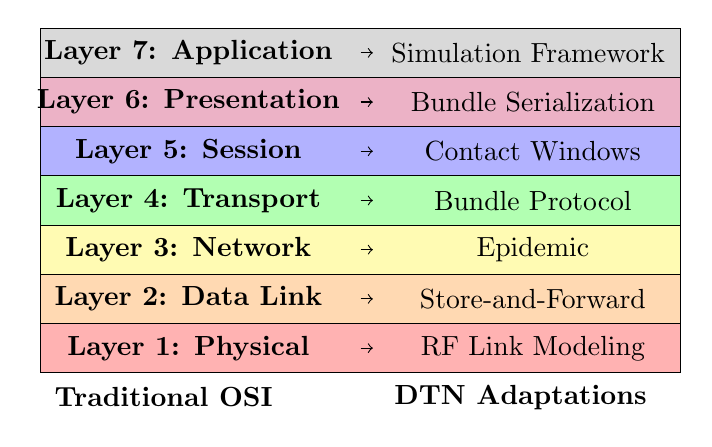
\begin{tikzpicture}[scale=0.625]
% OSI Layers
\foreach \i/\layer/\color in {
    1/Physical/red!30,
    2/Data Link/orange!30,
    3/Network/yellow!30,
    4/Transport/green!30,
    5/Session/blue!30,
    6/Presentation/purple!30,
    7/Application/gray!30
} {
    \draw[fill=\color] (0,\i-1) rectangle (13,\i);
    \node at (3,\i-0.5) {\textbf{Layer \i: \layer}};
}

% DTN Adaptations
\foreach \i/\adaptation in {
    1/RF Link Modeling,
    2/Store-and-Forward,
    3/Epidemic/PRoPHET/Spray-Wait,
    4/Bundle Protocol,
    5/Contact Windows,
    6/Bundle Serialization,
    7/Simulation Framework
} {
    \node[align=left] at (10,\i-0.5) {\adaptation};
    \draw[->] (6.5,\i-0.5) -- (6.75,\i-0.5);
}

\node at (2.5,-0.5) {\textbf{Traditional OSI}};
\node at (9.75,-0.5) {\textbf{DTN Adaptations}};
\end{tikzpicture}
\caption{OSI Model Adaptations in DTN Simulator}
\end{figure}

\subsection{Layer 1: Physical Layer}

\subsubsection{Implementation Components}
The Physical Layer in the DTN simulator handles RF communication modeling and satellite hardware simulation:

\begin{itemize}
    \item \textbf{File}: \texttt{orbital/contact\_prediction.py} (lines 59-287)
    \item \textbf{File}: \texttt{weather/weather\_model.py} (lines 41-114)
\end{itemize}

\subsubsection{RF Link Budget Implementation}
The \texttt{LinkBudget} class provides comprehensive RF modeling:

\begin{lstlisting}[language=Python]
class LinkBudget:
    def __init__(self):
        self.frequency_bands = {
            'S-band': 2.4e9,  # 2.4 GHz
            'C-band': 6.0e9,  # 6 GHz
            'Ku-band': 14.0e9, # 14 GHz
            'Ka-band': 20.0e9, # 20 GHz
            'V-band': 60.0e9   # 60 GHz
        }

    def calculate_link_budget(self, distance, frequency,
                            tx_power, antenna_gains):
        # Free space path loss (Friis equation)
        fspl = 20 * math.log10(distance) + \
               20 * math.log10(frequency) + 92.45

        # Total received power
        rx_power = tx_power + antenna_gains - fspl

        return rx_power
\end{lstlisting}

\subsubsection{Key Physical Layer Features}

\subsubsection{Frequency Band Support}
Multiple frequency bands with realistic propagation characteristics:
\begin{table}[H]
\centering
\begin{tabular}{@{}lcc@{}}
\toprule
\textbf{Band} & \textbf{Frequency} & \textbf{Applications} \\
\midrule
S-band & 2.4 GHz & Low data rate, robust \\
C-band & 6.0 GHz & Moderate data rate \\
Ku-band & 14.0 GHz & High data rate \\
Ka-band & 20.0 GHz & Very high data rate \\
V-band & 60.0 GHz & Experimental/research \\
\bottomrule
\end{tabular}
\caption{Supported RF Frequency Bands}
\end{table}

\subsubsection{Path Loss Calculations}
Free space path loss using the Friis transmission equation:
\begin{equation}
\text{FSPL}_{dB} = 20\log_{10}(4\pi d f / c)
\end{equation}

Implemented as:
\begin{equation}
\text{FSPL}_{dB} = 20\log_{10}(d) + 20\log_{10}(f) + 92.45
\end{equation}

\subsubsection{Atmospheric and Weather Effects}
Advanced modeling includes:
\begin{itemize}
    \item \textbf{Rain Attenuation}: ITU-R P.838 model implementation
    \item \textbf{Atmospheric Absorption}: Frequency-dependent oxygen/water vapor
    \item \textbf{Scintillation}: Amplitude fluctuations in satellite links
    \item \textbf{Cloud Attenuation}: Additional losses in cloudy conditions
\end{itemize}

\subsubsection{DTN-Specific Physical Layer Adaptations}

\subsubsection{Intermittent Connectivity Modeling}
Unlike traditional networks with persistent connections, the Physical Layer determines when communication is possible:

\begin{lstlisting}[language=Python]
def is_link_available(self, snr_db, min_snr_threshold=10.0):
    """Determine if RF link supports data transmission"""
    return snr_db >= min_snr_threshold

def calculate_data_rate(self, snr_linear, bandwidth):
    """Shannon capacity with coding efficiency"""
    shannon_capacity = bandwidth * math.log2(1 + snr_linear)
    return self.coding_efficiency * shannon_capacity
\end{lstlisting}

\subsubsection{Dynamic Link Quality}
Link quality varies continuously based on:
\begin{itemize}
    \item Satellite orbital position and distance
    \item Atmospheric conditions and weather
    \item Antenna pointing accuracy
    \item Interference levels
\end{itemize}

\subsection{Layer 2: Data Link Layer}

\subsubsection{Implementation Components}
Data Link Layer functionality is distributed across several components:

\begin{itemize}
    \item \textbf{File}: \texttt{orbital/contact\_prediction.py} (lines 175-204)
    \item \textbf{File}: \texttt{core/bundle.py} (lines 16-24)
\end{itemize}

\subsubsection{Frame Structure and Error Handling}
DTN bundles serve as Layer 2 frames with enhanced capabilities:

\begin{lstlisting}[language=Python]
class BundleFlags:
    IS_FRAGMENT = 0x01
    ADMIN_RECORD = 0x02
    DONT_FRAGMENT = 0x04
    CUSTODY_REQUESTED = 0x08
    DESTINATION_SINGLETON = 0x10
    APPLICATION_ACK_REQUESTED = 0x20
\end{lstlisting}

\subsubsection{Error Detection and Correction}
The simulator implements coding efficiency to model Forward Error Correction (FEC):

\begin{lstlisting}[language=Python]
def calculate_effective_data_rate(self, shannon_capacity):
    """Apply coding efficiency for error correction"""
    coding_efficiency = 0.75  # Typical for satellite links
    return shannon_capacity * coding_efficiency
\end{lstlisting}

\subsubsection{DTN-Specific Data Link Adaptations}

\subsubsection{Store-and-Forward Mechanism}
Traditional data link layers immediately forward or drop frames. DTN data link layer stores frames (bundles) when forwarding is impossible:

\begin{itemize}
    \item Bundles stored during link outages
    \item Automatic retransmission when links become available
    \item Buffer management with priority-based dropping
\end{itemize}

\subsubsection{Contact-Based Transmission}
Frame transmission occurs only during active contact windows:

\begin{lstlisting}[language=Python]
class ContactWindow:
    def __init__(self, source_id, target_id, start_time, end_time):
        self.source_id = source_id
        self.target_id = target_id
        self.start_time = start_time
        self.end_time = end_time
        self.data_rate = 0.0  # Calculated dynamically

    def can_transmit(self, current_time, bundle_size):
        """Check if bundle can be transmitted in remaining window"""
        if not (self.start_time <= current_time <= self.end_time):
            return False

        remaining_time = (self.end_time - current_time).total_seconds()
        transmission_time = bundle_size / self.data_rate

        return transmission_time <= remaining_time
\end{lstlisting}

\subsection{Layer 3: Network Layer}

\subsubsection{Implementation Components}
The Network Layer implements DTN-specific routing protocols:

\begin{itemize}
    \item \textbf{File}: \texttt{networking/routing/base\_router.py}
    \item \textbf{File}: \texttt{networking/routing/epidemic.py}
    \item \textbf{File}: \texttt{networking/routing/prophet.py}
    \item \textbf{File}: \texttt{networking/routing/spray\_and\_wait.py}
\end{itemize}

\subsubsection{DTN Addressing Scheme}
DTN uses Endpoint Identifiers (EIDs) instead of traditional IP addresses:

\begin{lstlisting}[language=Python]
@dataclass
class EndpointID:
    scheme: str  # e.g., "dtn"
    ssp: str     # Scheme-Specific Part (node identifier)

    def __str__(self):
        return f"{self.scheme}:{self.ssp}"
\end{lstlisting}

\subsubsection{Routing Algorithm Implementations}

\subsubsection{Epidemic Routing}
Floods network with bundle copies to maximize delivery probability:

\begin{lstlisting}[language=Python]
def should_forward(self, bundle, available_contacts, current_time):
    """Epidemic forwarding: replicate to all available neighbors"""
    for contact in available_contacts:
        # Calculate forwarding priority
        priority = self._calculate_forwarding_priority(
            bundle, contact, current_time
        )

        if priority > 0:
            return RoutingDecision(
                action="forward",
                next_hop=contact.target_id,
                priority=priority
            )

    return RoutingDecision(action="store")
\end{lstlisting}

\subsubsection{PRoPHET Routing}
Uses encounter history to predict delivery success:

\begin{lstlisting}[language=Python]
def _update_encounter_predictability(self, neighbor, encounter_time):
    """Update delivery predictability based on encounter"""
    old_pred = self.delivery_predictability.get(neighbor, 0.0)

    if old_pred == 0.0:
        new_pred = self.p_init  # First encounter
    else:
        # PRoPHET update equation
        new_pred = old_pred + (1 - old_pred) * self.p_encounter_max

    self.delivery_predictability[neighbor] = min(1.0, new_pred)
\end{lstlisting}

\subsubsection{Spray and Wait}
Limited replication with spray and wait phases:

\begin{lstlisting}[language=Python]
def should_forward(self, bundle, available_contacts, current_time):
    """Spray and Wait: controlled replication then direct delivery"""
    copies_remaining = self.bundle_copies[bundle.bundle_id]
    in_spray_phase = self.spray_phase[bundle.bundle_id]

    # Check for direct delivery
    if self._find_direct_contact(bundle.destination, available_contacts):
        return RoutingDecision(action="forward", priority=10.0)

    # Spray phase: distribute copies
    if in_spray_phase and copies_remaining > 1:
        copies_to_give = max(1, copies_remaining // 2)  # Binary spray
        return RoutingDecision(action="forward", copies=copies_to_give)

    # Wait phase: only direct delivery
    return RoutingDecision(action="store")
\end{lstlisting}

\subsubsection{DTN-Specific Network Layer Features}

\subsubsection{Opportunistic Routing}
Routes determined by contact opportunities rather than pre-computed paths:

\begin{itemize}
    \item No traditional route discovery protocols
    \item Forwarding decisions made per contact window
    \item Multiple routing strategies can coexist
\end{itemize}

\subsubsection{Store-and-Forward Routing}
Network layer stores packets when no forwarding opportunity exists:

\begin{itemize}
    \item Bundles stored at intermediate nodes
    \item Automatic forwarding when contacts become available
    \item Buffer management with aging and priority policies
\end{itemize}

\subsection{Layer 4: Transport Layer}

\subsubsection{Implementation Components}
The Transport Layer is implemented through the Bundle Protocol:

\begin{itemize}
    \item \textbf{File}: \texttt{core/bundle.py}
    \item \textbf{File}: \texttt{core/bundle.py} (lines 159-234): \texttt{BundleStore}
\end{itemize}

\subsubsection{Bundle Protocol Implementation}
DTN Bundle Protocol provides transport layer services:

\begin{lstlisting}[language=Python]
@dataclass
class Bundle:
    bundle_id: str
    source: EndpointID
    destination: EndpointID
    creation_timestamp: datetime
    lifetime: timedelta
    payload_size: int
    priority: int = 1
    flags: int = 0
    hop_count: int = 0

    def is_expired(self, current_time: datetime) -> bool:
        """Check if bundle has exceeded its lifetime"""
        age = current_time - self.creation_timestamp
        return age > self.lifetime

    @property
    def remaining_lifetime(self) -> timedelta:
        """Calculate remaining time before expiration"""
        age = datetime.now() - self.creation_timestamp
        return max(timedelta(0), self.lifetime - age)
\end{lstlisting}

\subsubsection{Reliability Mechanisms}

\subsubsection{Custody Transfer}
Hop-by-hop reliability mechanism:

\begin{lstlisting}[language=Python]
class CustodyManager:
    def request_custody(self, bundle, next_hop):
        """Request custody transfer to next hop"""
        if bundle.flags & BundleFlags.CUSTODY_REQUESTED:
            # Store bundle until custody acknowledgment
            self.custody_bundles[bundle.bundle_id] = bundle
            return True
        return False

    def accept_custody(self, bundle_id, from_node):
        """Accept custody and send acknowledgment"""
        ack = self.create_custody_ack(bundle_id)
        self.send_admin_record(ack, from_node)
\end{lstlisting}

\subsubsection{Lifetime Management}
Bundles have explicit lifetimes with aging policies:

\begin{lstlisting}[language=Python]
class BundleStore:
    def age_bundles(self, current_time):
        """Remove expired bundles and update statistics"""
        expired_bundles = []

        for bundle in self.stored_bundles:
            if bundle.is_expired(current_time):
                expired_bundles.append(bundle)

        for bundle in expired_bundles:
            self.remove_bundle(bundle.bundle_id)
            self.metrics.bundles_expired += 1
\end{lstlisting}

\subsubsection{DTN-Specific Transport Layer Features}

\subsubsection{Long-Term Storage}
Unlike traditional transport protocols, DTN supports extended storage:

\begin{itemize}
    \item Bundles may be stored for hours or days
    \item Persistent storage across system restarts
    \item Graceful handling of storage constraints
\end{itemize}

\subsubsection{Multiple Delivery Semantics}
DTN supports various delivery guarantees:

\begin{itemize}
    \item Best-effort delivery (no guarantees)
    \item Custody transfer (hop-by-hop reliability)
    \item End-to-end acknowledgments
    \item Priority-based delivery
\end{itemize}

\subsection{Layer 5: Session Layer}

\subsubsection{Implementation Components}
Session Layer manages contact windows and communication sessions:

\begin{itemize}
    \item \textbf{File}: \texttt{orbital/contact\_prediction.py} (lines 18-44)
    \item \textbf{File}: \texttt{simulation/realtime\_engine.py} (lines 244-302)
\end{itemize}

\subsubsection{Contact Window Management}
Sessions are defined by satellite contact windows:

\begin{lstlisting}[language=Python]
class ContactWindow:
    def __init__(self, source_id, target_id, start_time, end_time):
        self.source_id = source_id
        self.target_id = target_id
        self.start_time = start_time
        self.end_time = end_time
        self.elevation = 0.0
        self.azimuth = 0.0
        self.range_km = 0.0
        self.data_rate = 0.0

    @property
    def duration_seconds(self):
        """Contact window duration in seconds"""
        return (self.end_time - self.start_time).total_seconds()

    def is_active(self, current_time):
        """Check if contact window is currently active"""
        return self.start_time <= current_time <= self.end_time
\end{lstlisting}

\subsubsection{Session Establishment and Management}
Contact prediction provides session scheduling:

\begin{lstlisting}[language=Python]
class ContactPredictor:
    def predict_contacts(self, satellite_state, ground_station,
                        start_time, duration):
        """Predict communication opportunities"""
        contacts = []
        current_time = start_time
        end_time = start_time + duration

        while current_time < end_time:
            elevation, azimuth, range_km = self.calculate_geometry(
                satellite_state, ground_station, current_time
            )

            if elevation > self.elevation_mask:
                # Start of contact window
                contact_start = current_time

                # Find end of contact window
                while elevation > self.elevation_mask:
                    current_time += self.time_step
                    elevation, _, _ = self.calculate_geometry(
                        satellite_state, ground_station, current_time
                    )

                contact = ContactWindow(
                    source_id=satellite_state.satellite_id,
                    target_id=ground_station.id,
                    start_time=contact_start,
                    end_time=current_time
                )
                contacts.append(contact)

            current_time += self.time_step

        return contacts
\end{lstlisting}

\subsubsection{DTN-Specific Session Layer Features}

\subsubsection{Predictive Session Management}
Sessions are predicted using orbital mechanics:

\begin{itemize}
    \item Contact windows calculated in advance
    \item Session scheduling based on satellite orbits
    \item Dynamic session quality assessment
\end{itemize}

\subsubsection{Intermittent Session Handling}
Sessions have natural start and end times:

\begin{itemize}
    \item Automatic session termination when satellites go below horizon
    \item Session resumption on next satellite pass
    \item Multi-hop virtual sessions through store-and-forward
\end{itemize}

\subsection{Layer 6: Presentation Layer}

\subsubsection{Implementation Components}
Presentation Layer handles data serialization and encoding:

\begin{itemize}
    \item \textbf{File}: \texttt{core/bundle.py} (lines 117-156)
    \item \textbf{File}: \texttt{api/models/base\_models.py}
\end{itemize}

\subsubsection{Bundle Serialization}
Bundles must be serialized for storage and transmission:

\begin{lstlisting}[language=Python]
class Bundle:
    def to_dict(self) -> Dict[str, Any]:
        """Serialize bundle to dictionary for storage/transmission"""
        return {
            'bundle_id': self.bundle_id,
            'source': str(self.source),
            'destination': str(self.destination),
            'creation_timestamp': self.creation_timestamp.isoformat(),
            'lifetime_seconds': self.lifetime.total_seconds(),
            'payload_size': self.payload_size,
            'priority': self.priority,
            'flags': self.flags,
            'hop_count': self.hop_count
        }

    @classmethod
    def from_dict(cls, data: Dict[str, Any]) -> 'Bundle':
        """Deserialize bundle from dictionary"""
        return cls(
            bundle_id=data['bundle_id'],
            source=EndpointID.parse(data['source']),
            destination=EndpointID.parse(data['destination']),
            creation_timestamp=datetime.fromisoformat(
                data['creation_timestamp']
            ),
            lifetime=timedelta(seconds=data['lifetime_seconds']),
            payload_size=data['payload_size'],
            priority=data.get('priority', 1),
            flags=data.get('flags', 0),
            hop_count=data.get('hop_count', 0)
        )
\end{lstlisting}

\subsubsection{API Data Models}
External representation through Pydantic models:

\begin{lstlisting}[language=Python]
class SimulationResponse(BaseModel):
    simulation_id: str
    name: str
    status: str
    constellation: str
    routing_algorithm: str
    created_at: datetime

    class Config:
        json_encoders = {
            datetime: lambda v: v.isoformat()
        }
\end{lstlisting}

\subsubsection{DTN-Specific Presentation Features}

\subsubsection{Persistent Encoding}
Bundles must remain valid during long storage periods:

\begin{itemize}
    \item Platform-independent serialization format
    \item Version-tolerant deserialization
    \item Metadata preservation across hops
\end{itemize}

\subsubsection{Cross-Platform Compatibility}
Bundles may traverse different satellite platforms:

\begin{itemize}
    \item Standardized bundle format
    \item Endian-neutral encoding
    \item Time zone independent timestamps
\end{itemize}

\subsection{Layer 7: Application Layer}

\subsubsection{Implementation Components}
Application Layer provides user-facing services:

\begin{itemize}
    \item \textbf{File}: \texttt{api/app.py}
    \item \textbf{File}: \texttt{api/routers/}
    \item \textbf{File}: \texttt{core/simulation.py}
\end{itemize}

\subsubsection{REST API Services}
FastAPI application provides management interface:

\begin{lstlisting}[language=Python]
@app.post("/api/v2/simulation/create")
async def create_simulation(request: CreateSimulationRequest):
    """Create new DTN simulation"""
    simulation = Simulation(
        name=request.name,
        constellation_id=request.constellation_id,
        routing_algorithm=request.routing_algorithm,
        duration=request.duration,
        ground_stations=request.ground_stations
    )

    simulation_id = await simulation_manager.create(simulation)

    return CreateSimulationResponse(
        simulation_id=simulation_id,
        message="Simulation created successfully"
    )

@app.get("/api/v2/simulation/{simulation_id}/metrics")
async def get_metrics(simulation_id: str):
    """Get simulation performance metrics"""
    metrics = await simulation_manager.get_metrics(simulation_id)

    return SimulationMetricsResponse(
        delivery_ratio=metrics.delivery_ratio,
        average_delay=metrics.average_delay,
        overhead_ratio=metrics.overhead_ratio,
        buffer_utilization=metrics.buffer_utilization
    )
\end{lstlisting}

\subsubsection{Simulation Framework}
High-level application for DTN research:

\begin{lstlisting}[language=Python]
class ExperimentFramework:
    def run_comparative_experiment(self, config):
        """Run experiment comparing multiple routing algorithms"""
        results = {}

        for algorithm in config.routing_algorithms:
            # Run multiple iterations for statistical validity
            algorithm_results = []

            for iteration in range(config.iterations):
                simulation = self.create_simulation(
                    constellation=config.constellation,
                    routing_algorithm=algorithm,
                    duration=config.duration
                )

                result = self.run_simulation(simulation)
                algorithm_results.append(result)

            # Calculate statistics
            results[algorithm] = self.calculate_statistics(
                algorithm_results
            )

        return ExperimentReport(results)
\end{lstlisting}

\subsubsection{DTN-Specific Application Features}

\subsubsection{Delay-Tolerant Management}
Applications designed for asynchronous operations:

\begin{itemize}
    \item Asynchronous simulation control
    \item Long-running experiment management
    \item Progress tracking and status updates
\end{itemize}

\subsubsection{DTN Research Tools}
Specialized applications for DTN analysis:

\begin{itemize}
    \item Routing algorithm comparison framework
    \item Performance metrics collection and analysis
    \item Constellation design optimization tools
    \item Contact plan visualization and analysis
\end{itemize}

\subsection{Cross-Layer Integration}

\subsubsection{Key Interactions}

\subsubsection{Physical Network Layer}
RF link quality directly affects routing decisions:

\begin{lstlisting}[language=Python]
def calculate_forwarding_priority(self, bundle, contact):
    """Priority based on link quality and routing algorithm"""
    base_priority = contact.data_rate / 100.0

    # Boost for direct delivery
    if contact.target_id == bundle.destination.ssp:
        base_priority += 10.0

    # Reduce for poor link quality
    if contact.snr_db < 15.0:
        base_priority *= 0.5

    return base_priority
\end{lstlisting}

\subsubsection{Data Link Transport Layer}
Contact duration limits affect bundle transmission:

\begin{lstlisting}[language=Python]
def can_transmit_bundle(self, bundle, contact_window):
    """Check if bundle can be transmitted in available time"""
    transmission_time = bundle.payload_size / contact_window.data_rate
    remaining_time = contact_window.remaining_duration()

    return transmission_time <= remaining_time
\end{lstlisting}

\subsubsection{Network Session Layer}
Routing algorithms use contact prediction:

\begin{lstlisting}[language=Python]
def update_routing_info(self, contact_plan):
    """Update routing state with predicted contacts"""
    for contact in contact_plan:
        if self.is_neighbor_contact(contact):
            # Update delivery predictability for PRoPHET
            self._update_encounter_predictability(
                contact.target_id, contact.start_time
            )
\end{lstlisting}

\subsubsection{DTN Design Principles}

\subsubsection{Store-and-Forward Architecture}
All layers support intermittent connectivity:

\begin{itemize}
    \item Physical: Links may be unavailable for extended periods
    \item Data Link: Frames stored when transmission impossible
    \item Network: Packets stored at intermediate nodes
    \item Transport: End-to-end delivery despite long delays
\end{itemize}

\subsubsection{Opportunistic Communication}
Layers adapt to dynamic connectivity:

\begin{itemize}
    \item Contact-based transmission scheduling
    \item Adaptive routing based on contact opportunities
    \item Dynamic quality assessment and adaptation
\end{itemize}

\subsubsection{Resource Management}
All layers include resource constraints:

\begin{itemize}
    \item Physical: Power and bandwidth limitations
    \item Data Link: Buffer management for frames
    \item Network: Memory constraints for routing tables
    \item Transport: Storage limits for bundles
\end{itemize}

This comprehensive OSI analysis demonstrates how the DTN simulator adapts traditional networking concepts to handle the unique challenges of satellite communications, including intermittent connectivity, long delays, and resource constraints, while maintaining architectural clarity through the layered model.

\

% Conclusion
\section{Conclusion}

\subsection{Project Summary}

The DTN Simulator represents a comprehensive implementation of delay-tolerant networking principles specifically designed for satellite communications research. Through realistic orbital mechanics, advanced routing protocols, and detailed RF modeling, the simulator provides researchers with a powerful tool for studying DTN performance in space-based networks.

\subsection{Key Achievements}

\subsubsection{Technical Accomplishments}
\begin{itemize}
    \item \textbf{Realistic Simulation Environment}: Implementation of SGP4/SDP4 orbital propagation with accurate satellite positioning
    \item \textbf{Advanced Routing Protocols}: Complete implementation of Epidemic, PRoPHET, and Spray-and-Wait algorithms with performance comparison
    \item \textbf{Comprehensive RF Modeling}: Detailed link budget calculations including weather effects and atmospheric attenuation
    \item \textbf{Interactive Visualization}: Real-time 3D visualization with military-style command center interface
    \item \textbf{Scalable Architecture}: Support for large satellite constellations with efficient computation
\end{itemize}

\subsubsection{Research Contributions}
\begin{itemize}
    \item \textbf{Protocol Comparison Framework}: Systematic evaluation of DTN routing algorithms in realistic scenarios
    \item \textbf{Weather Impact Analysis}: Quantitative assessment of environmental effects on satellite communications
    \item \textbf{Constellation Optimization}: Tools for evaluating satellite network designs and ground station placement
    \item \textbf{Performance Benchmarking}: Standardized metrics for DTN protocol evaluation
\end{itemize}

\subsection{Educational Value}

The simulator serves as an excellent educational tool for:

\begin{itemize}
    \item \textbf{Networking Concepts}: Hands-on experience with DTN principles and store-and-forward networking
    \item \textbf{Orbital Mechanics}: Practical application of satellite orbital dynamics and contact prediction
    \item \textbf{RF Engineering}: Understanding of link budgets, path loss, and communication systems
    \item \textbf{Protocol Design}: Analysis of routing algorithm trade-offs and performance characteristics
\end{itemize}

\subsection{Future Enhancements}

\subsubsection{Near-Term Improvements}
\begin{itemize}
    \item \textbf{Additional Routing Protocols}: MaxProp, RAPID, and other advanced DTN algorithms
    \item \textbf{Security Features}: Bundle encryption, authentication, and secure routing
    \item \textbf{Mobile Ground Stations}: Support for ships, aircraft, and vehicle-based terminals
    \item \textbf{Inter-Satellite Links}: Direct satellite-to-satellite communication modeling
\end{itemize}

\subsubsection{Long-Term Roadmap}
\begin{itemize}
    \item \textbf{Machine Learning Integration}: AI-based routing decisions and network optimization
    \item \textbf{Real-Time Hardware Integration}: Connection to actual satellite tracking systems
    \item \textbf{Multi-Constellation Support}: Simultaneous simulation of multiple satellite networks
    \item \textbf{Advanced Visualization}: Virtual reality interface for immersive network exploration
\end{itemize}

\subsection{Impact and Applications}

\subsubsection{Research Applications}
\begin{itemize}
    \item Satellite constellation design optimization
    \item DTN routing algorithm development and evaluation
    \item Ground station network planning
    \item Emergency communication system design
    \item Interplanetary communication protocol research
\end{itemize}

\subsubsection{Commercial Potential}
\begin{itemize}
    \item Satellite operator network planning tools
    \item Emergency response communication systems
    \item Remote area connectivity solutions
    \item Maritime and aviation communication networks
\end{itemize}

\subsection{Acknowledgments}

This project represents the collaborative effort of researchers dedicated to advancing delay-tolerant networking and satellite communications. The simulator builds upon decades of research in DTN protocols, orbital mechanics, and RF engineering, providing a platform for continued innovation in space-based networking.

The comprehensive implementation demonstrates the practical application of theoretical concepts, bridging the gap between academic research and real-world satellite communication systems. Through this work, we aim to contribute to the advancement of robust, efficient communication networks that can operate reliably in the challenging environment of space.

\subsection{Final Remarks}

The DTN Simulator stands as a testament to the power of simulation in understanding complex distributed systems. By providing a realistic, comprehensive environment for studying delay-tolerant networks, this tool enables researchers and engineers to explore the frontiers of space-based communication systems.

As satellite constellations become increasingly important for global connectivity, tools like this simulator will play a crucial role in designing and optimizing the communication networks of the future. The project's open architecture and extensible design ensure that it will continue to evolve and support the growing needs of the DTN research community.

Through careful implementation of mathematical models, realistic system constraints, and user-friendly interfaces, the DTN Simulator provides both immediate utility for current research and a foundation for future innovations in delay-tolerant networking and satellite communications.

\

% Bibliography
\begin{thebibliography}{99}

\bibitem{fall03}
Fall, K., \& Farrell, S. (2008).
\textit{DTN: An architectural retrospective}.
IEEE Journal on Selected Areas in Communications, 26(5), 828-836.

\bibitem{cerf07}
Cerf, V., Burleigh, S., Hooke, A., Torgerson, L., Durst, R., Scott, K., ... \& Weiss, H. (2007).
\textit{Delay-tolerant networking architecture}.
RFC 4838.

\bibitem{vahdat00}
Vahdat, A., \& Becker, D. (2000).
\textit{Epidemic routing for partially connected ad hoc networks}.
Technical Report CS-2000-06, Duke University.

\bibitem{lindgren03}
Lindgren, A., Doria, A., \& Schelén, O. (2003).
\textit{Probabilistic routing in intermittently connected networks}.
ACM SIGMOBILE mobile computing and communications review, 7(3), 19-20.

\bibitem{spyropoulos05}
Spyropoulos, T., Psounis, K., \& Raghavendra, C. S. (2005).
\textit{Spray and wait: an efficient routing scheme for intermittently connected mobile networks}.
In Proceedings of the 2005 ACM SIGCOMM workshop on Delay-tolerant networking (pp. 252-259).

\bibitem{kelso07}
Kelso, T. S. (2007).
\textit{Validation of SGP4 and IS-GPS-200D against GPS precision ephemerides}.
In Proceedings of the AAS/AIAA Astrodynamics Conference.

\bibitem{vallado13}
Vallado, D., Crawford, P., Hujsak, R., \& Kelso, T. S. (2006).
\textit{Revisiting spacetrack report\# 3}.
In AIAA/AAS astrodynamics specialist conference and exhibit (p. 6753).

\bibitem{itu838}
ITU-R Recommendation P.838-3. (2005).
\textit{Specific attenuation model for rain for use in prediction methods}.
International Telecommunication Union.

\bibitem{burleigh10}
Burleigh, S., Hooke, A., Torgerson, L., Fall, K., Cerf, V., Durst, B., ... \& Weiss, H. (2003).
\textit{Delay-tolerant networking: an approach to interplanetary Internet}.
IEEE Communications Magazine, 41(6), 128-136.

\bibitem{akyildiz04}
Akyildiz, I. F., Akan, Ö. B., Chen, C., Fang, J., \& Su, W. (2003).
\textit{InterPlaNetary Internet: state-of-the-art and research challenges}.
Computer Networks, 43(2), 75-112.

\end{thebibliography}

\end{document}
